% Pour faire une référence d'une annexe
% (Annexe \ref{sec:nomsection} page~\pageref{sec:nomsection})

\section{Deux transcriptions de la pièce \textit{Reflets de l'ombre}, Carmine E. Cella, 2013}
\label{sec:refletsDeLOmbre}
\begin{figure}[H]
	\centering
	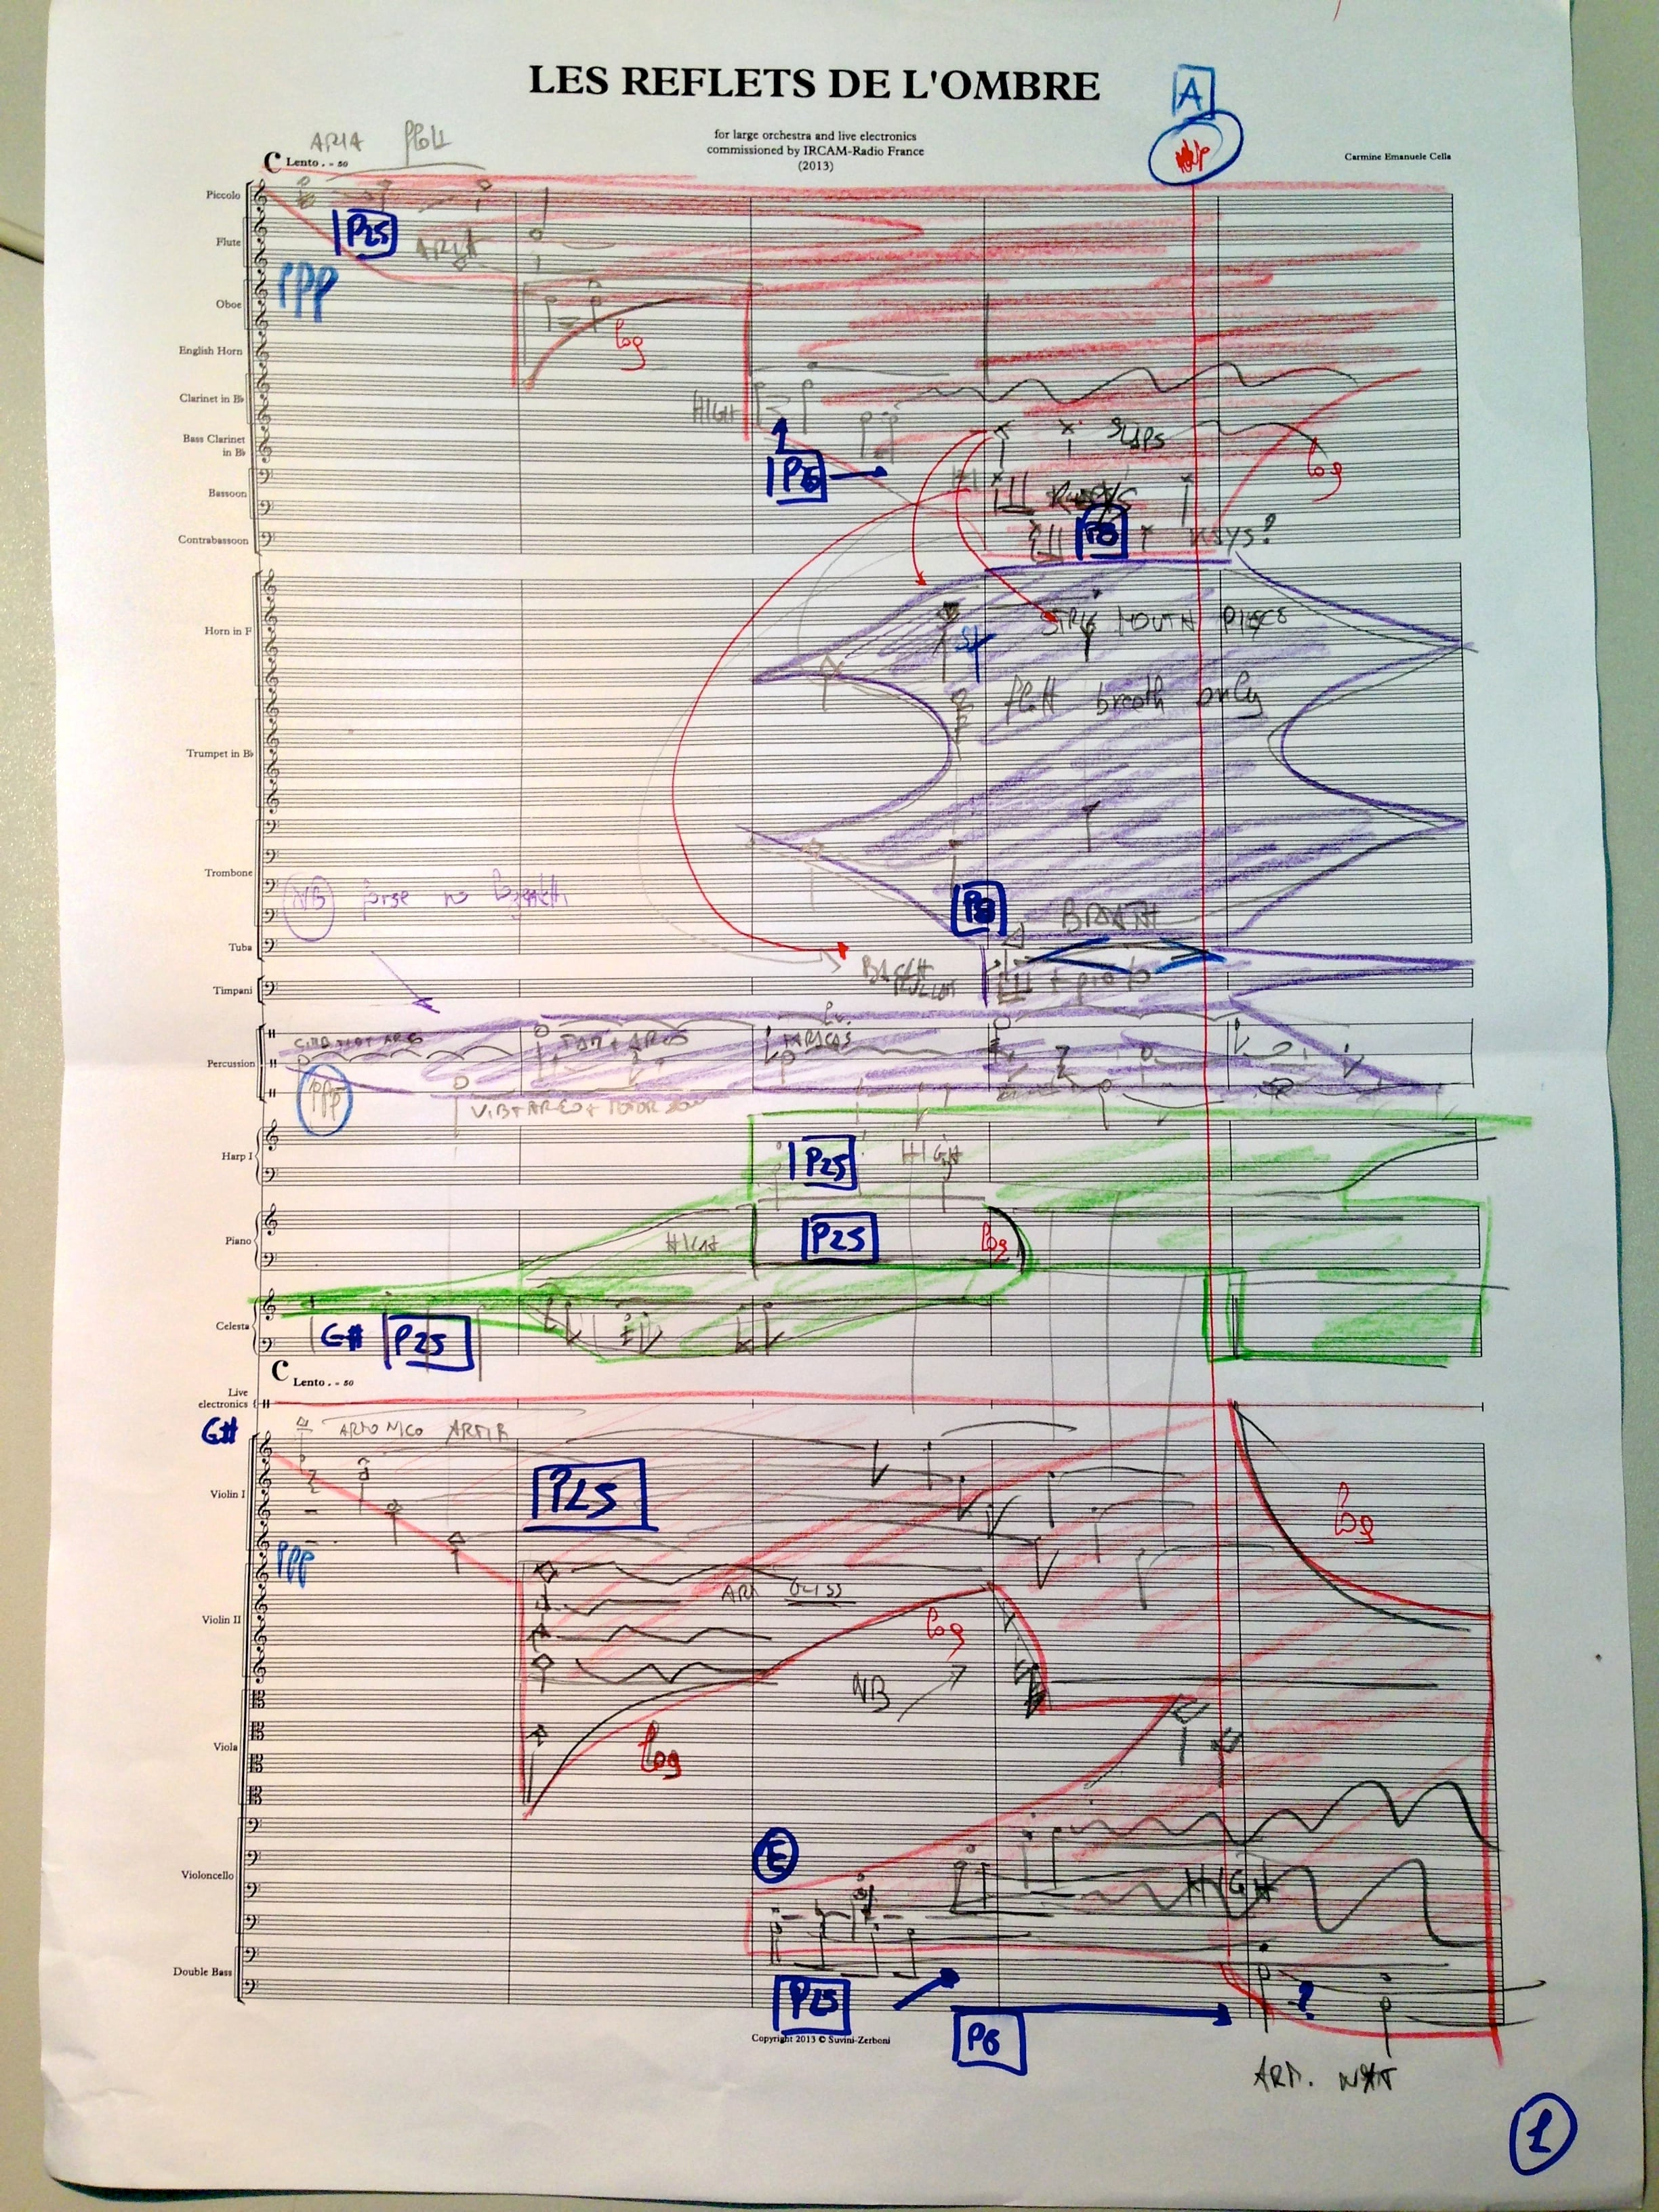
\includegraphics[keepaspectratio=true, width=0.8\textwidth]{Annexes/i/refletsDeLOmbreFantaisie.jpg}
	\caption{Extrait d'une première version de \textit{Reflets de l'ombre} par Carmine E. Cella}
	\medskip
	\small
	\textit{Cette première version représente la pièce en termes de variations du timbre du son.
	La musique y est notée de manière quasi morphologique, avec quelques ajouts de symboles de la gravure standard.}	
	\label{fig:refletsDeLOmbreFantaisie}
\end{figure}

\begin{figure}[H]
	\centering
	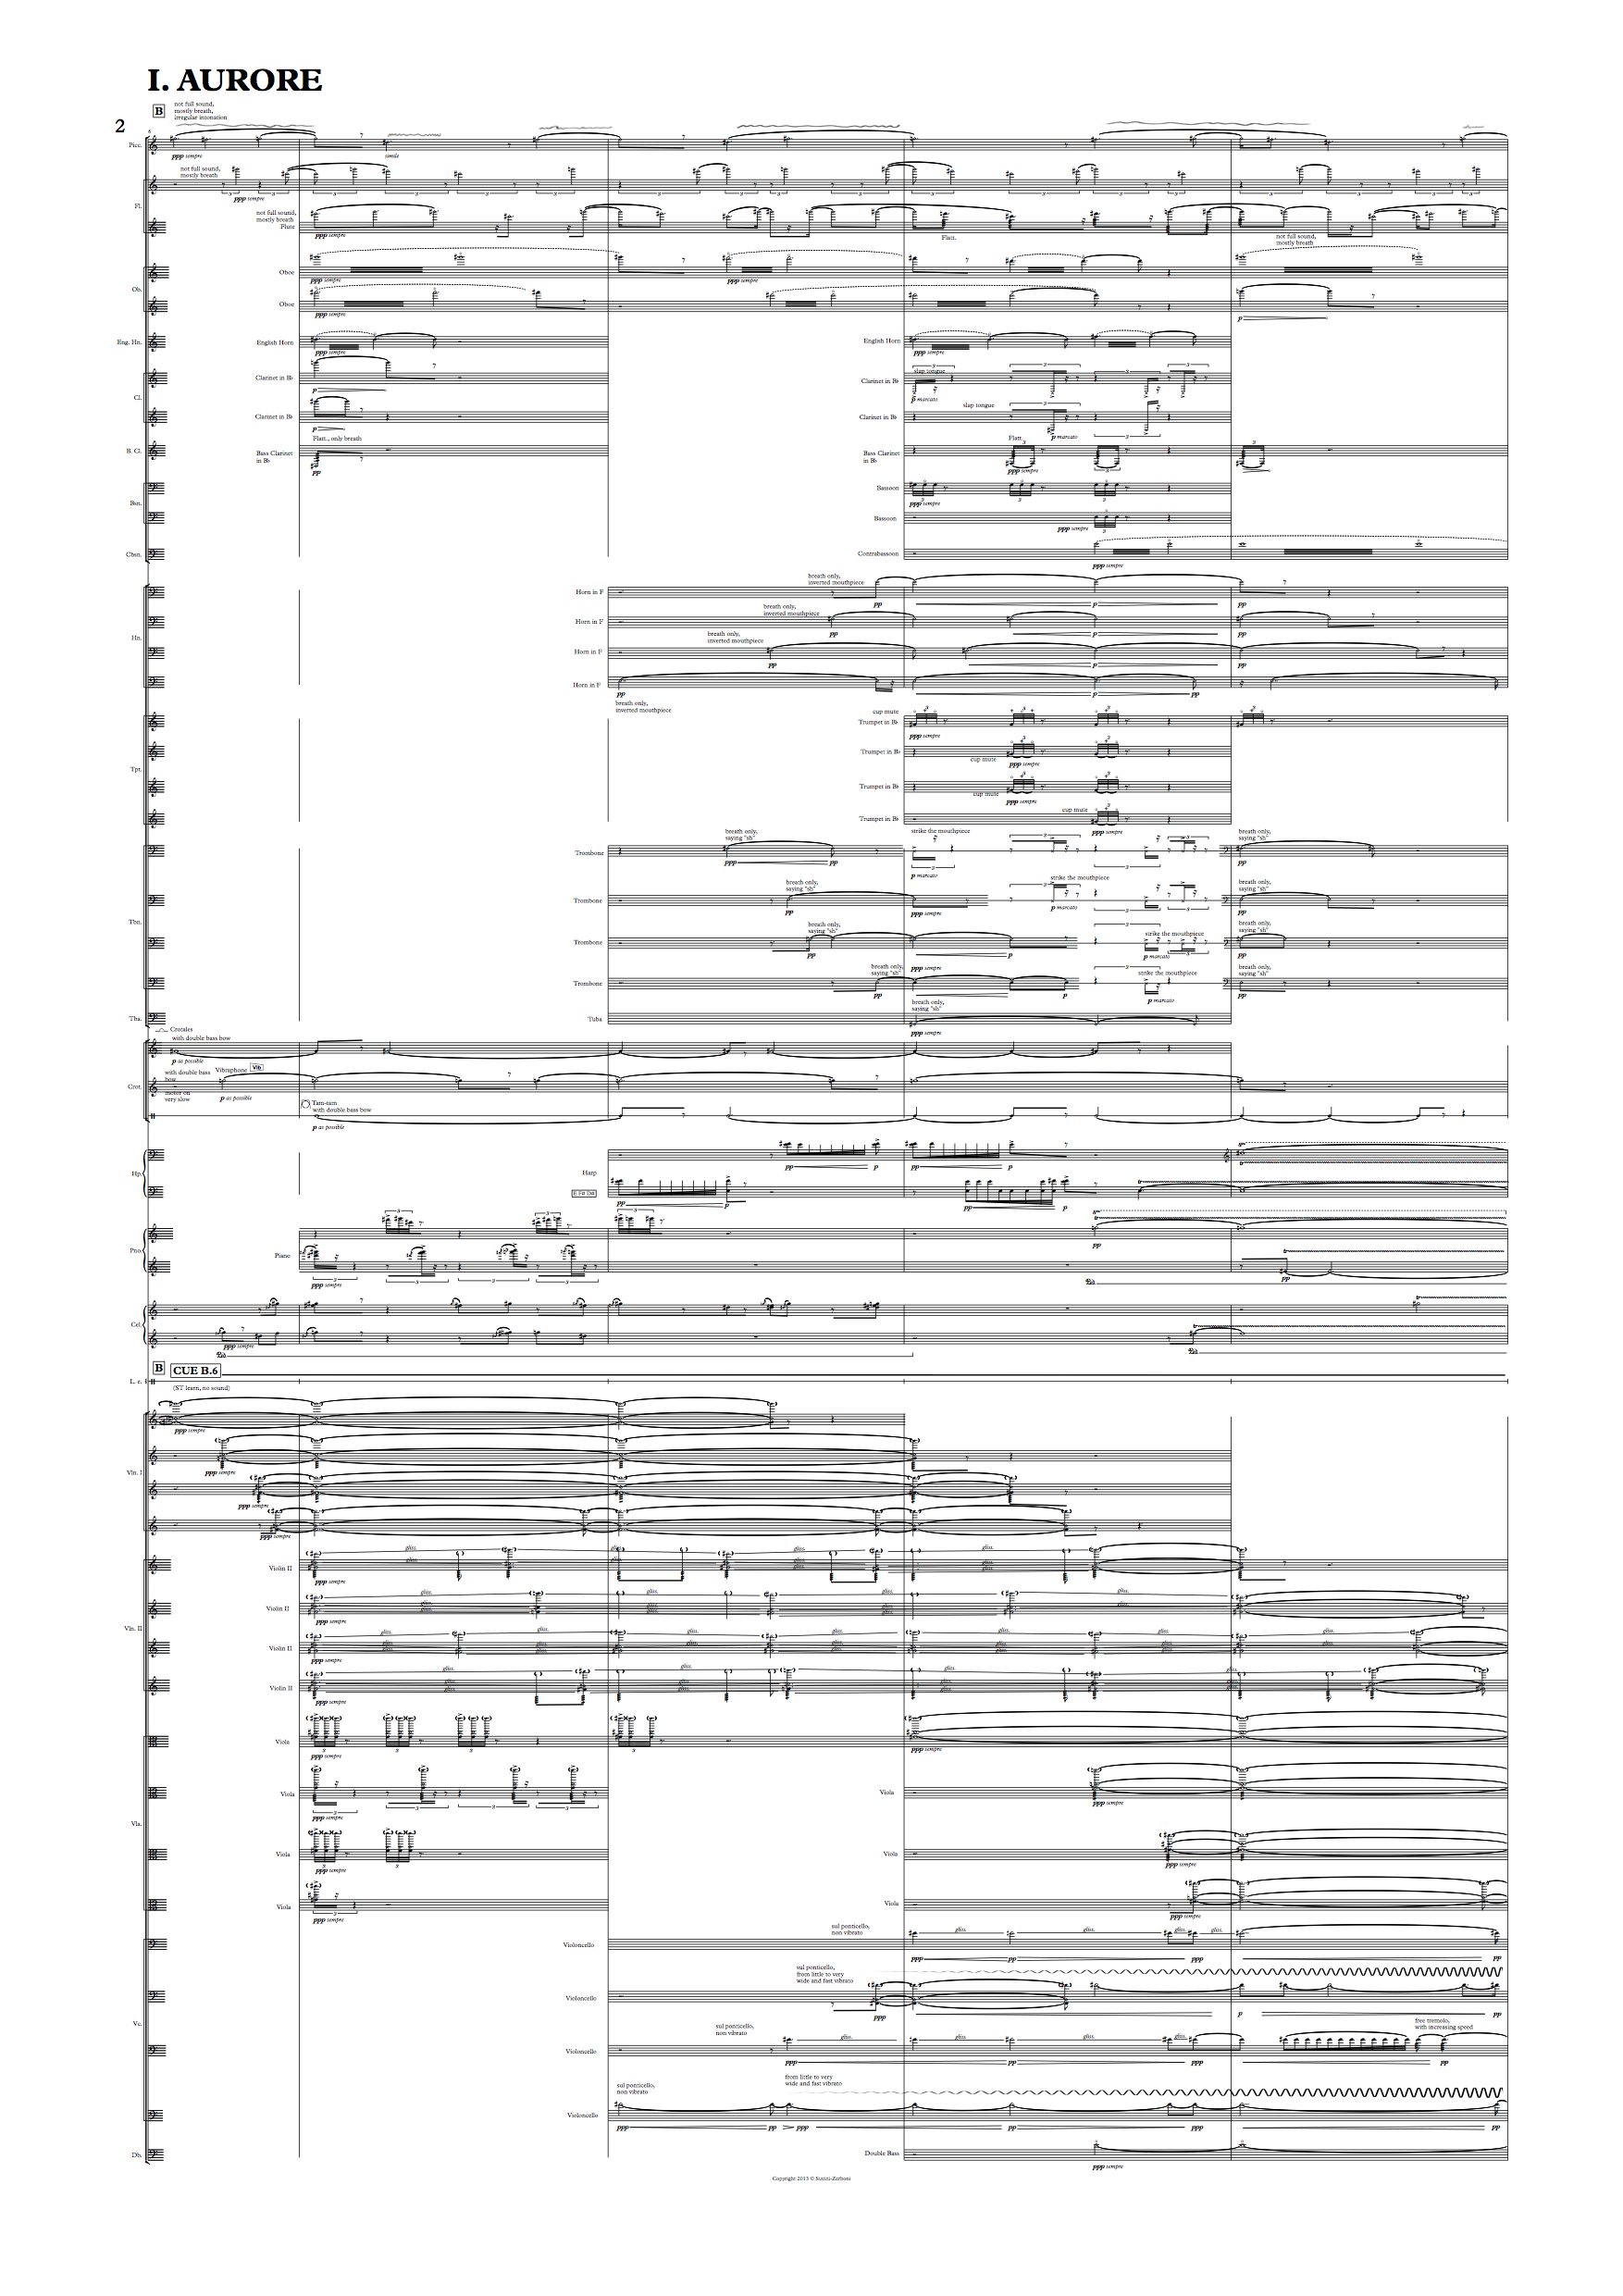
\includegraphics[keepaspectratio=true, width=0.9\textwidth]{Annexes/i/refletsDeLOmbreReel.png}
	\caption{Extrait d'une version éxecutée par un orchestre de \textit{Reflets de l'ombre} par Carmine E. Cella}
	\label{fig:refletsDeLOmbreReel}
	\medskip
	\small
	\it
	Cette version de la pièce, qui est destinée à l'orchestre exécutant, a été remaniée vis à vis de la version de la figure \ref{fig:refletsDeLOmbreFantaisie}. Cependant, les formes du son se retrouvent même dans cette transcription plus littérale.
\end{figure}
\clearpage

\section{Exemple de texte neumé}
\label{sec:exempleTexteNeume}
\begin{figure}[H]
	\centering
	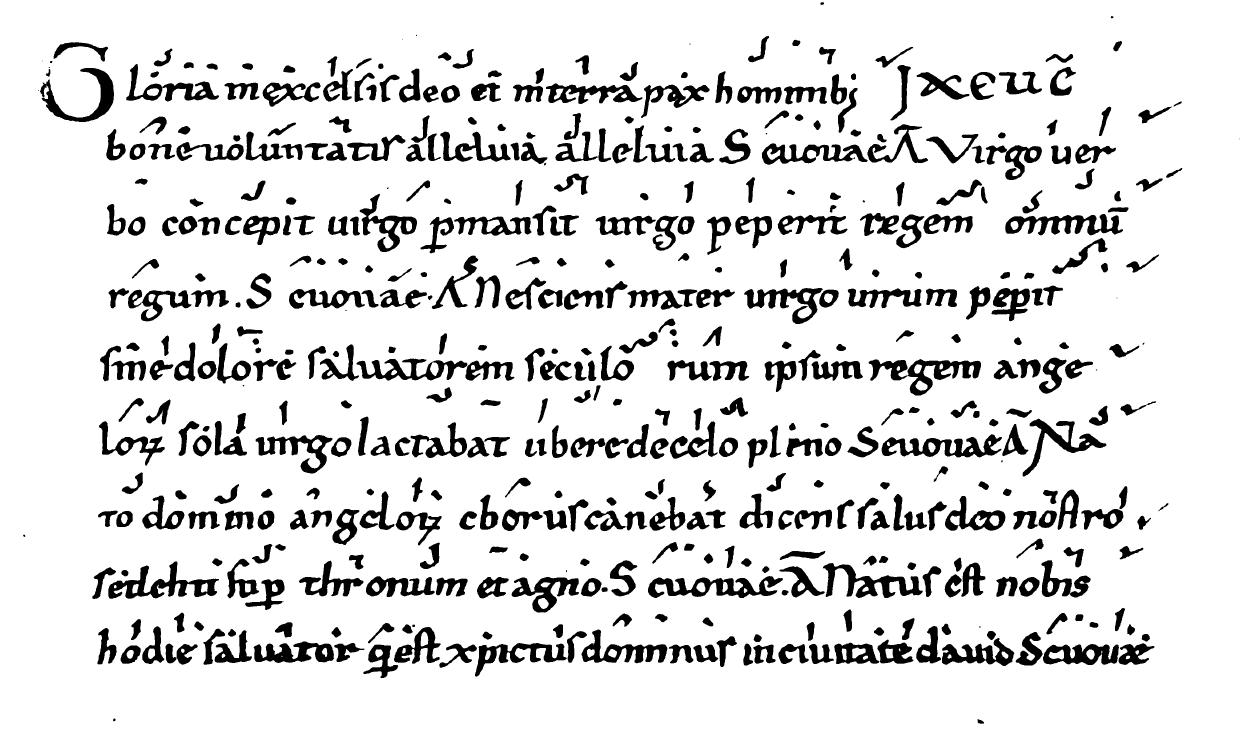
\includegraphics[keepaspectratio=true, width=\textwidth]{Annexes/i/neumes.jpg}
	\caption{Exemple de texte neumé}
	\medskip
	\small	
	Source : 1774, Martin Gerbert, \textit{De cantu et musica sacra a prima Ecclesiae aetate usque ad praesens Tempus}, St. Blasien, Typis San-Blasianis, t. I, t. II. - \it Les neumes sont inscrits au-dessus des mots du chant liturgique (ici le chant Gloria de l'ordinaire de la messe). Les inflexions de la voix sont notées par des symboles assez simples, combinaisons de courbes et points essentiellement. L'idée étant seulement de donner un repère visuel au chantre (moine exécutant la liturgie), qui connaît déjà par cœur la pièce.
	\label{fig:neumes}
\end{figure}
\clearpage

\section{La notation carrée}
\label{sec:exempleNotationCarree}
\begin{figure}[H]
	\centering
	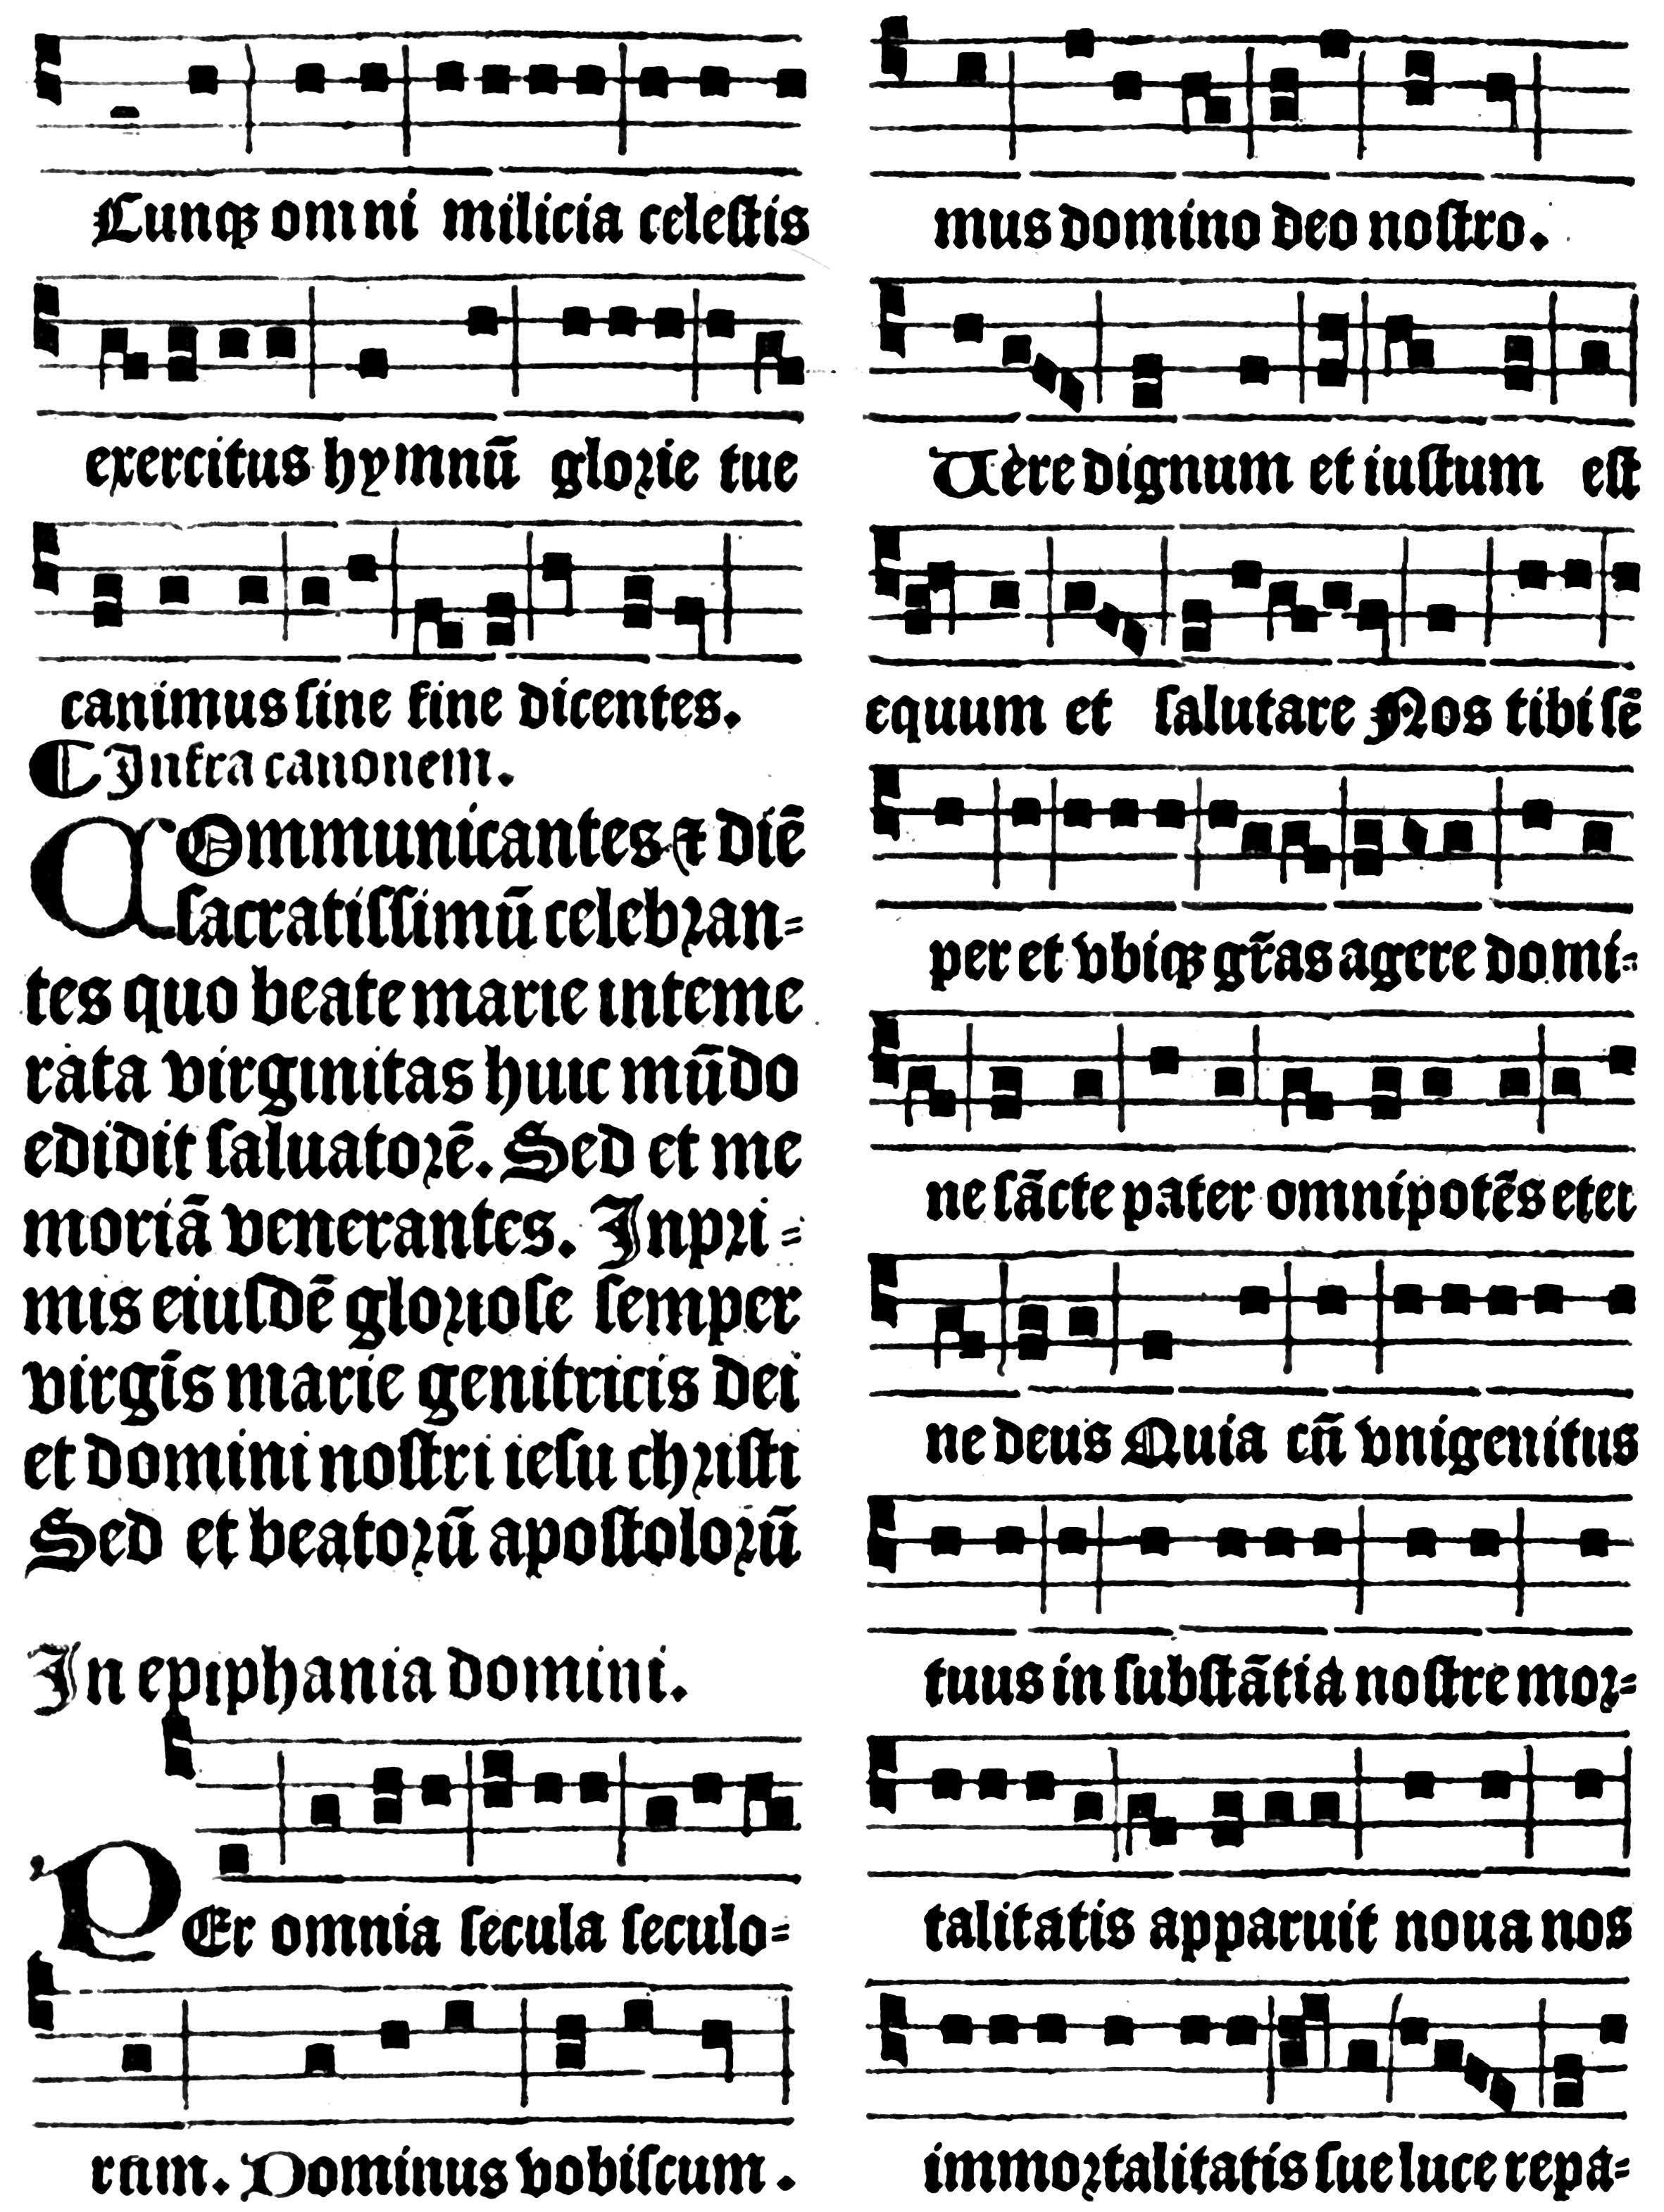
\includegraphics[keepaspectratio=true, width=0.8\textwidth]{Annexes/i/notationCarree.jpg}
	\caption{Exemple de notation carrée "imprimée"}
	\medskip
	\small
	Source : 1499, Jean Highman, \textit{Missale Leodiense}, Paris - \textit{Les notes sont représentées en notation carrée toujours au-dessus du texte chanté. L'exemple donné ci-dessus est une partition imprimée de la fin du XVème siècle, prouvant que les pratiques notationnelles perdurent même au-delà des périodes définies.}
	\label{fig:notationCarree}
\end{figure}
\clearpage

\section{La notation épurée de l'époque baroque}
\label{sec:exempleMusiqueBaroque}
\begin{figure}[H]
	\centering
	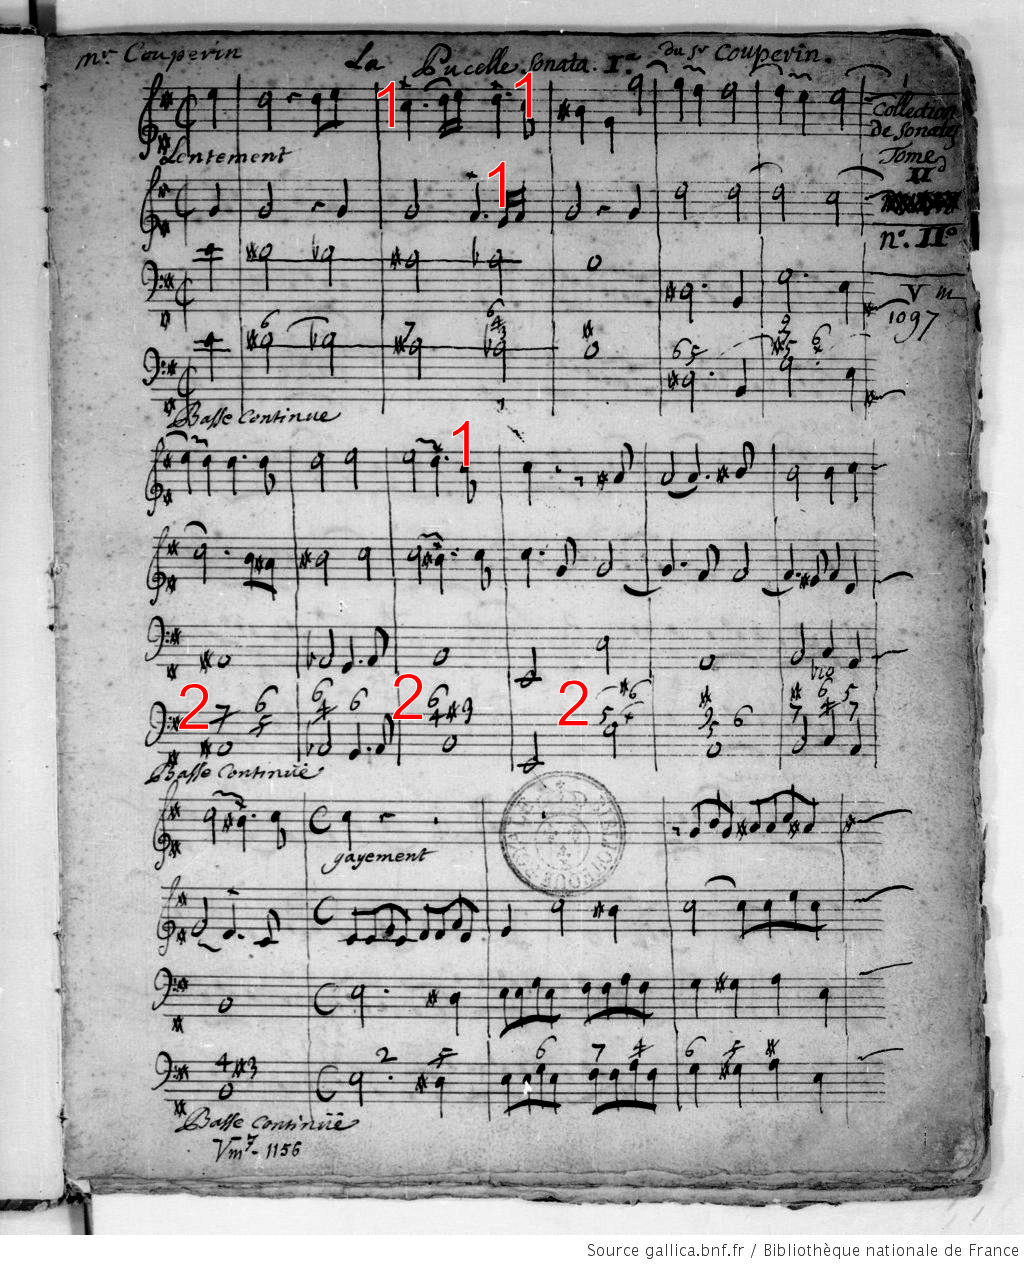
\includegraphics[keepaspectratio=true, width=\textwidth]{Annexes/i/exempleMusiqueBaroque.jpeg}
	\caption{Extrait de la pièce \textit{La Pucelle}, par François Couperin, 1690-1710}
	\medskip
	\small
	\it
	Source : Bibliothèque nationale de France, département Musique, VM7-1156.
	En 1, des symboles au-dessus des notes donnant des indications d'interprétation pour le soliste (+, vaguelettes). En 2, les numéros au-dessus des notes de la voix la plus basse (le morceau est une système à quatre voix) indiquent l'harmonie. C'est une manière de simplifier la notation des accords. 	
	\label{fig:exempleMusiqueBaroque}
\end{figure}
\clearpage

\section{La notation de l'interprétation}
\label{sec:exempleNotationInterpretation}
\begin{figure}[H]
	\centering
	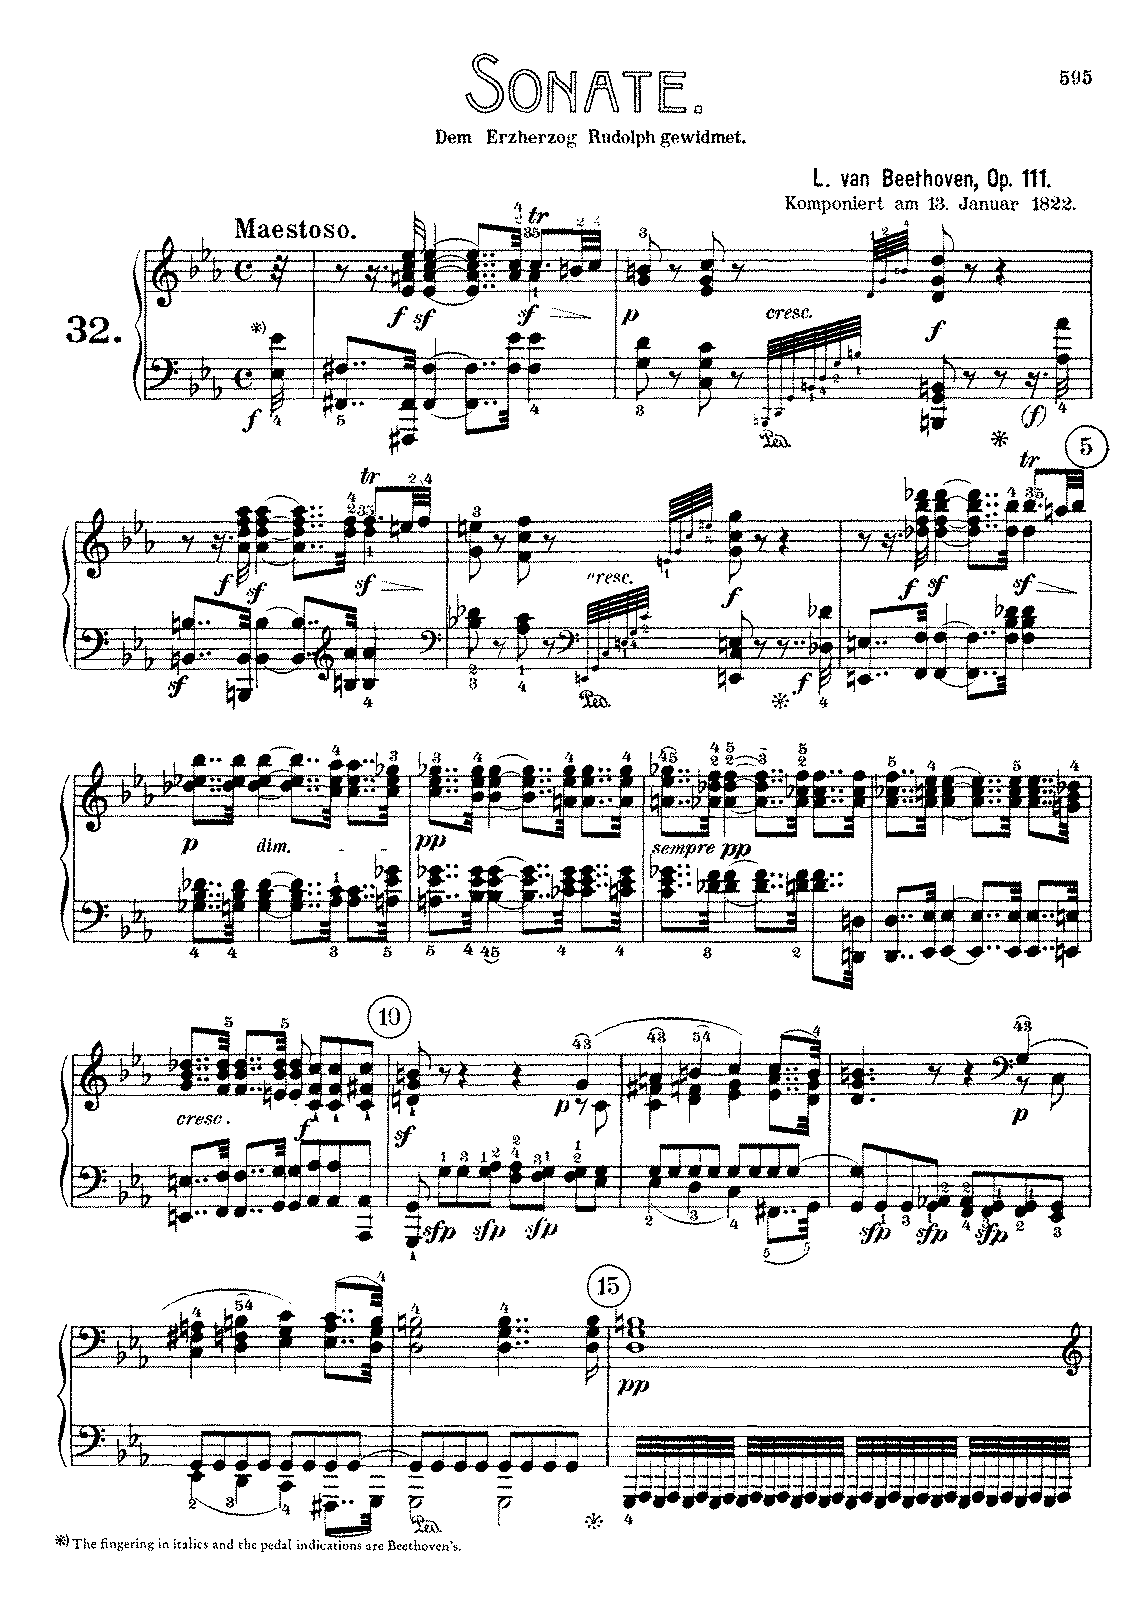
\includegraphics[keepaspectratio=true, width=0.9\textwidth]{Annexes/i/exempleNotationInterpretation.png}
	\caption{Extrait de la \textit{Sonate pour piano, N.32, Opus 111}, Ludwig van Beethoven, 1821-1822}
	\label{fig:exempleNotationInterpretation}	
	\medskip
	\small
	\it
	Source : IMSLP, Petrucci Music Library. En 1, des numéros indiquant le doigté à utiliser pour la pièce.
	En 2, des indications de nuances de jeu : pp pour pianissimo, sfp pour sforzando-piano. En 3, symbole indiquant l'utilisation de la pédale du piano pour jouer la phrase. 	
\end{figure}

\section{Exemple de partition graphique du XXème siècle}
\label{sec:exempleAnestisLogothetis}
\begin{figure}[H]
	\centering
	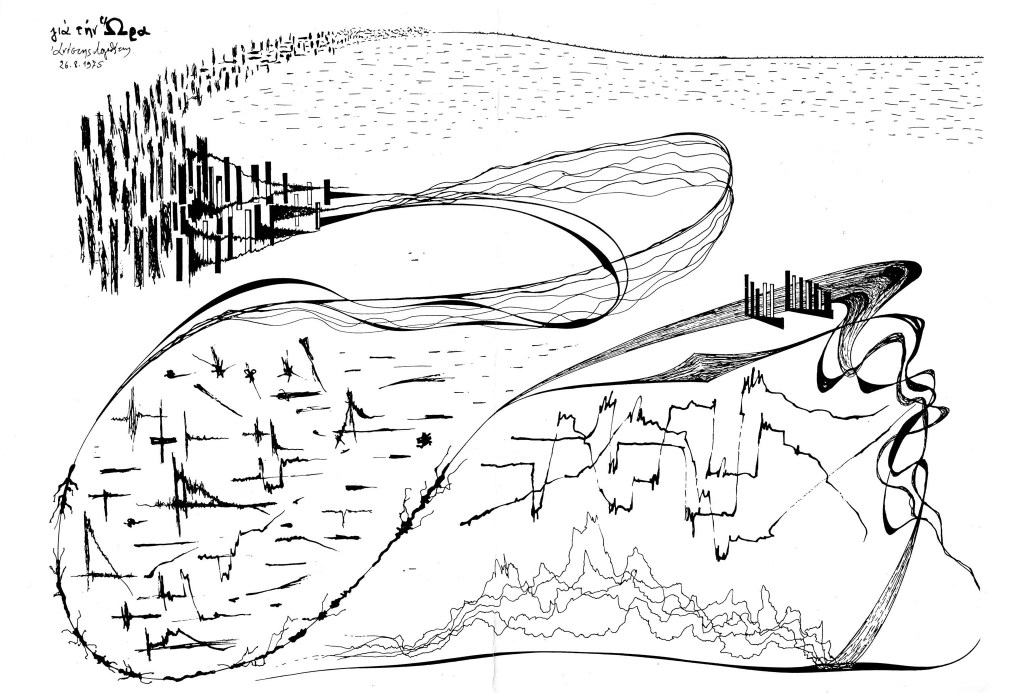
\includegraphics[keepaspectratio=true, width=0.9\textwidth]{Annexes/i/exempleAnestisLogothetis.jpg}
	\caption{Partition de \textit{Ghia tin ora} (Pour l'heure), Anestis Logothetis, 1975} 	
	\label{fig:exempleAnestisLogothetis}
	\medskip
	\small
	\it	
	Source : \url{http://schlachten.org/artist/logothetis-ensemble/}. Dans cette partition de la deuxième moitié du XXème siècle les nuages de points et les courbes sont préférés à l'expression sur la portée. L'influence de la musique électroacoustique sur la notation musicale se traduit par une représentation proche de la morphologie du son (représentation de la forme d'ondes).
\end{figure}
\clearpage

\rotatebox{90}{
\begin{minipage}{0.95\textheight}
	\section{Notation du geste dans la musique contemporaine}
	\label{sec:exempleKarimHaddad}
	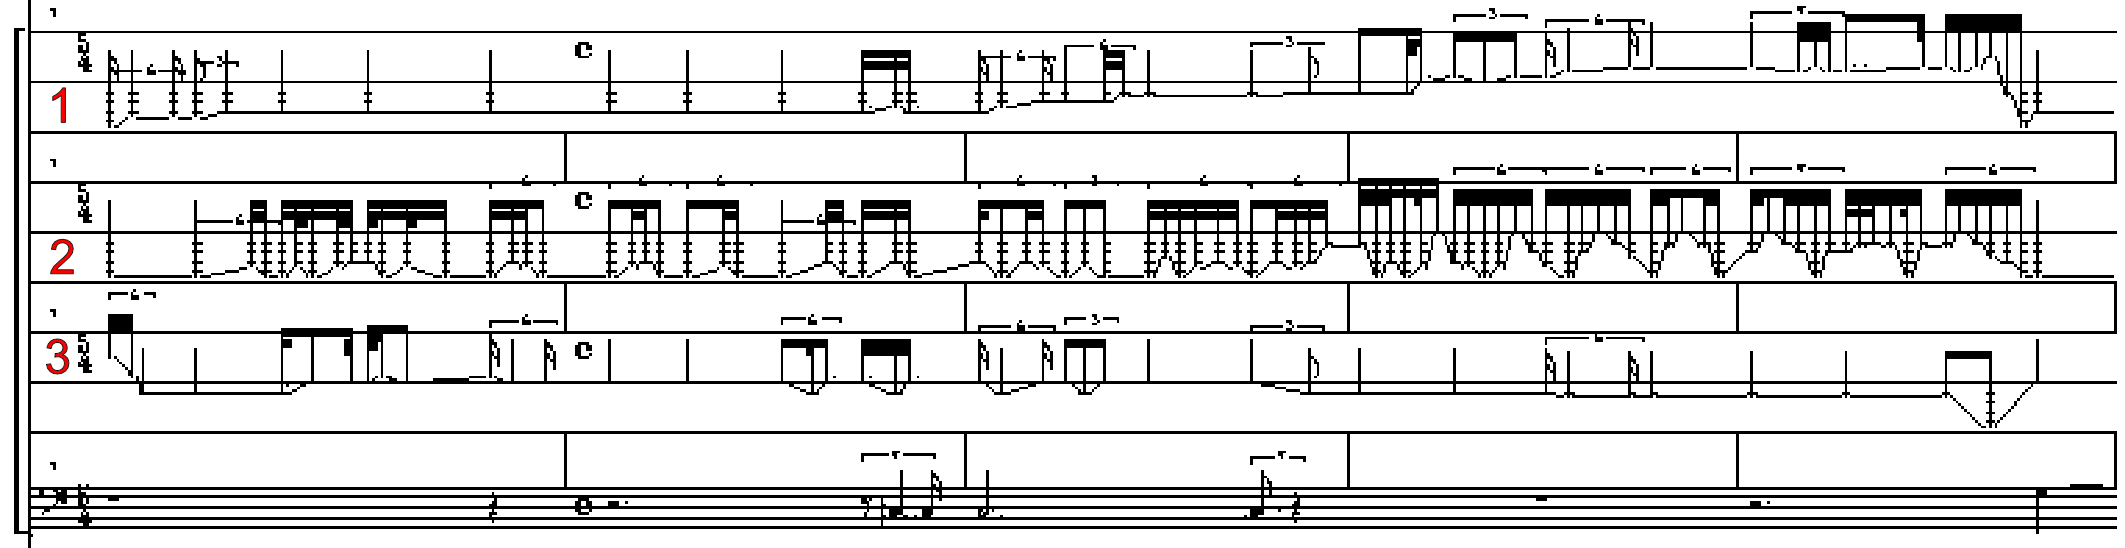
\includegraphics[keepaspectratio=true, width=\textwidth, height=\textheight]{Annexes/i/exempleKarimHaddad.png}
	\captionof{figure}{Fragment de la pièce \textit{In lieblicher Blaue…}, Karim Haddad}
	\label{fig:exempleKarimHaddad}    	
    	\medskip
	\small
	En 1, notation de la pression de l'archet sur la contrebasse. En 2, notation du placement de l'archet sur la contrebasse. En 3, notation de la vitesse de déplacement de l'archet sur la contrebasse.
\end{minipage}}
\clearpage

\rotatebox{90}{
\begin{minipage}{0.95\textheight}
	\section{Notation de la spatialisation du son dans la musique contemporaine}
	\label{sec:exempleAlirezaFarhang}
	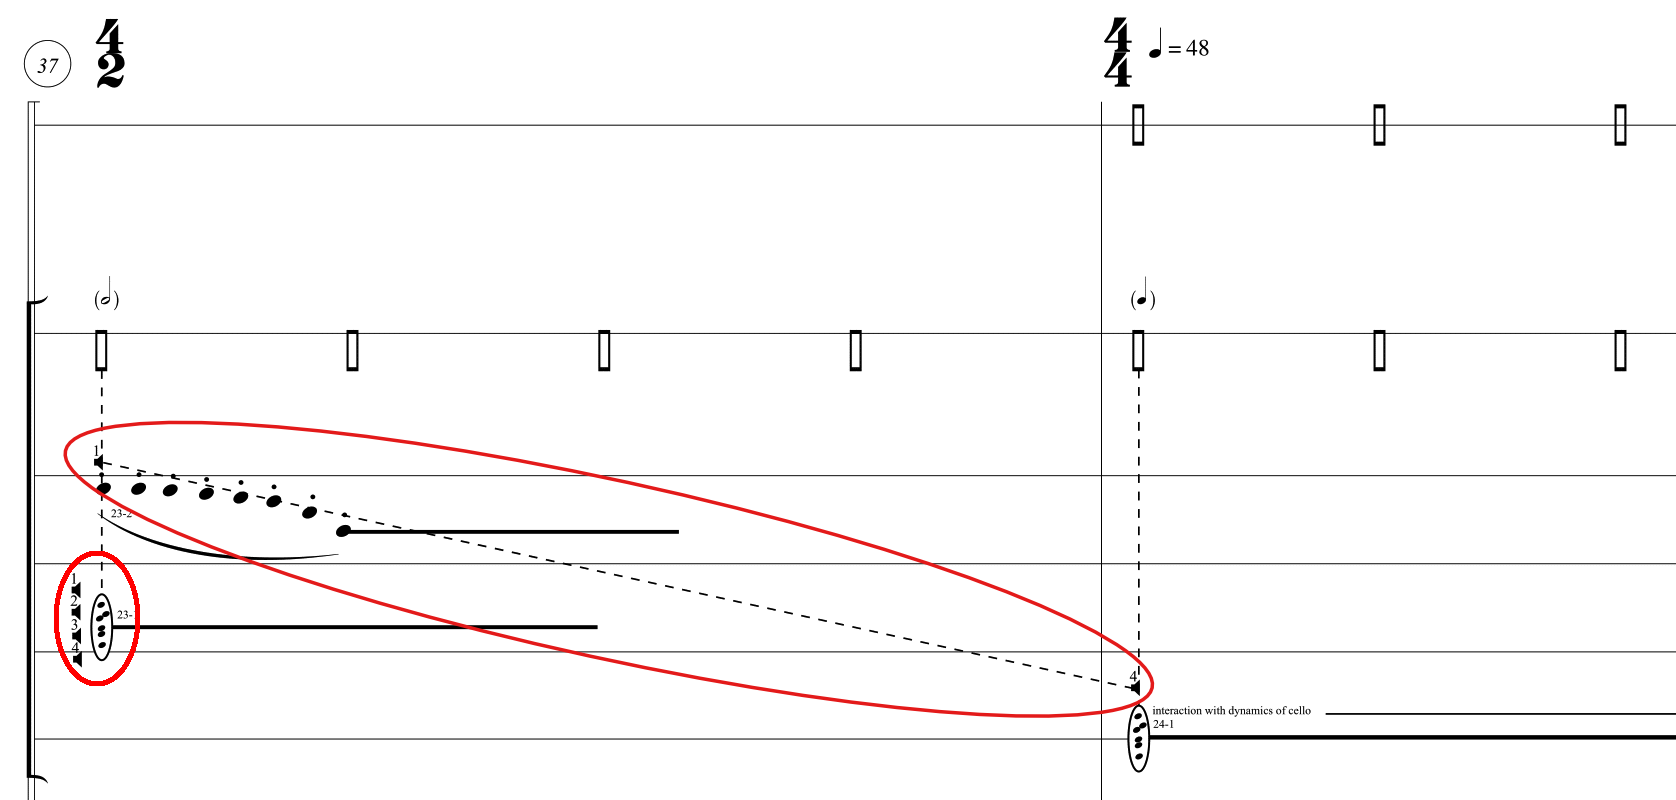
\includegraphics[keepaspectratio=true, width=\textwidth]{Annexes/i/exempleAlirezaFarhang.png}
	\captionof{figure}{Fragment de la pièce \textit{Tak Sîm}, Alireza Farhang, 2012}
	\label{fig:exempleAlirezaFarhang}	
	\medskip
	\small
	\it
	En rouge, la description des trajectoires de déplacement du son dans le système de diffusion de la pièce.
\end{minipage}}
\clearpage

\rotatebox{90}{
\begin{minipage}{0.95\textheight}
	\section{Notation des effets appliqués au son dans la musique contemporaine}
	\label{sec:exempleStockhausen}
	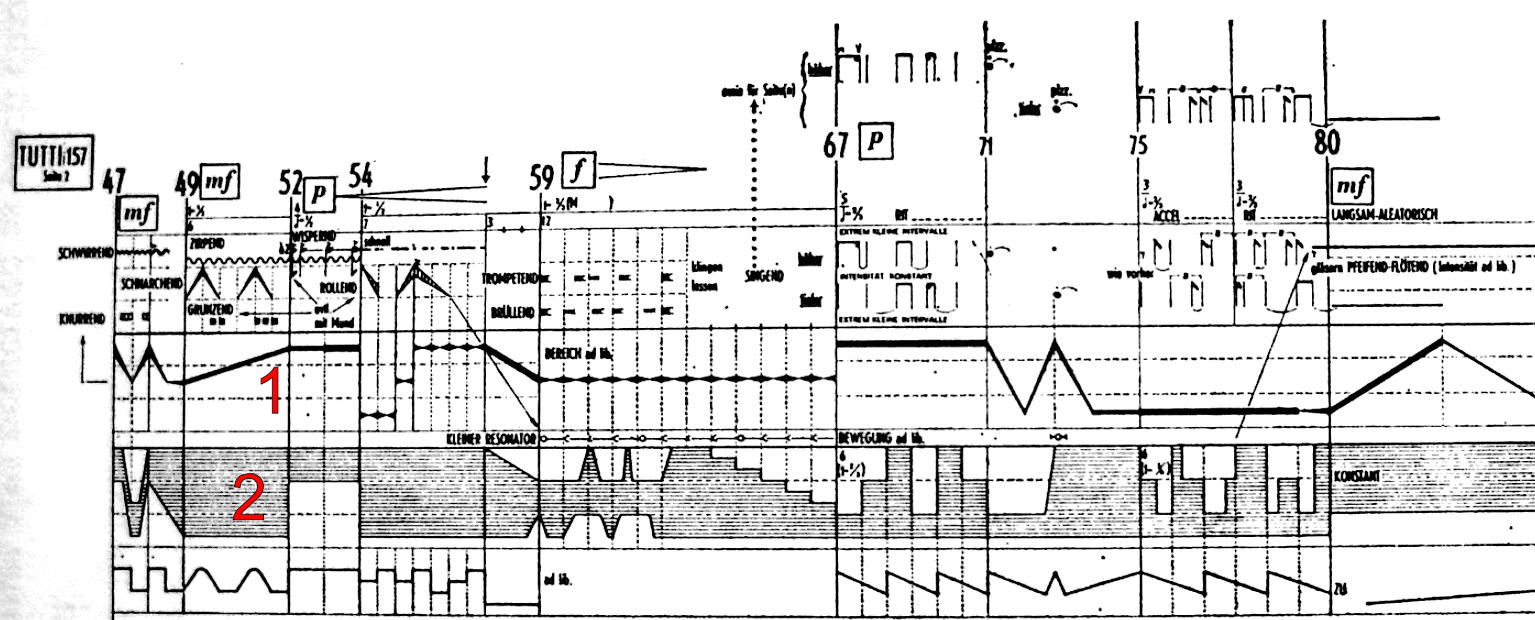
\includegraphics[keepaspectratio=true, width=\textwidth]{Annexes/i/exempleStockhausen.jpg}
	\captionof{figure}{Fragment de la pièce \textit{Tutti 157}, Karlheinz Stockhausen, 1964}
	\label{fig:exempleStockhausen}	
	\medskip
	\small
	\it
	En 1, la variation de la distance entre le micro et le gong. En 2, la variation de la bande de fréquence du son par filtrage.
\end{minipage}}
\clearpage

\section{Schéma complet de branchement pour la pièce \textit{Fluoresce}, Rama Gottfried, 2012}				\label{sec:schemaInstallationFluoresceComplet}
\begin{figure}[H]
	\centering	
	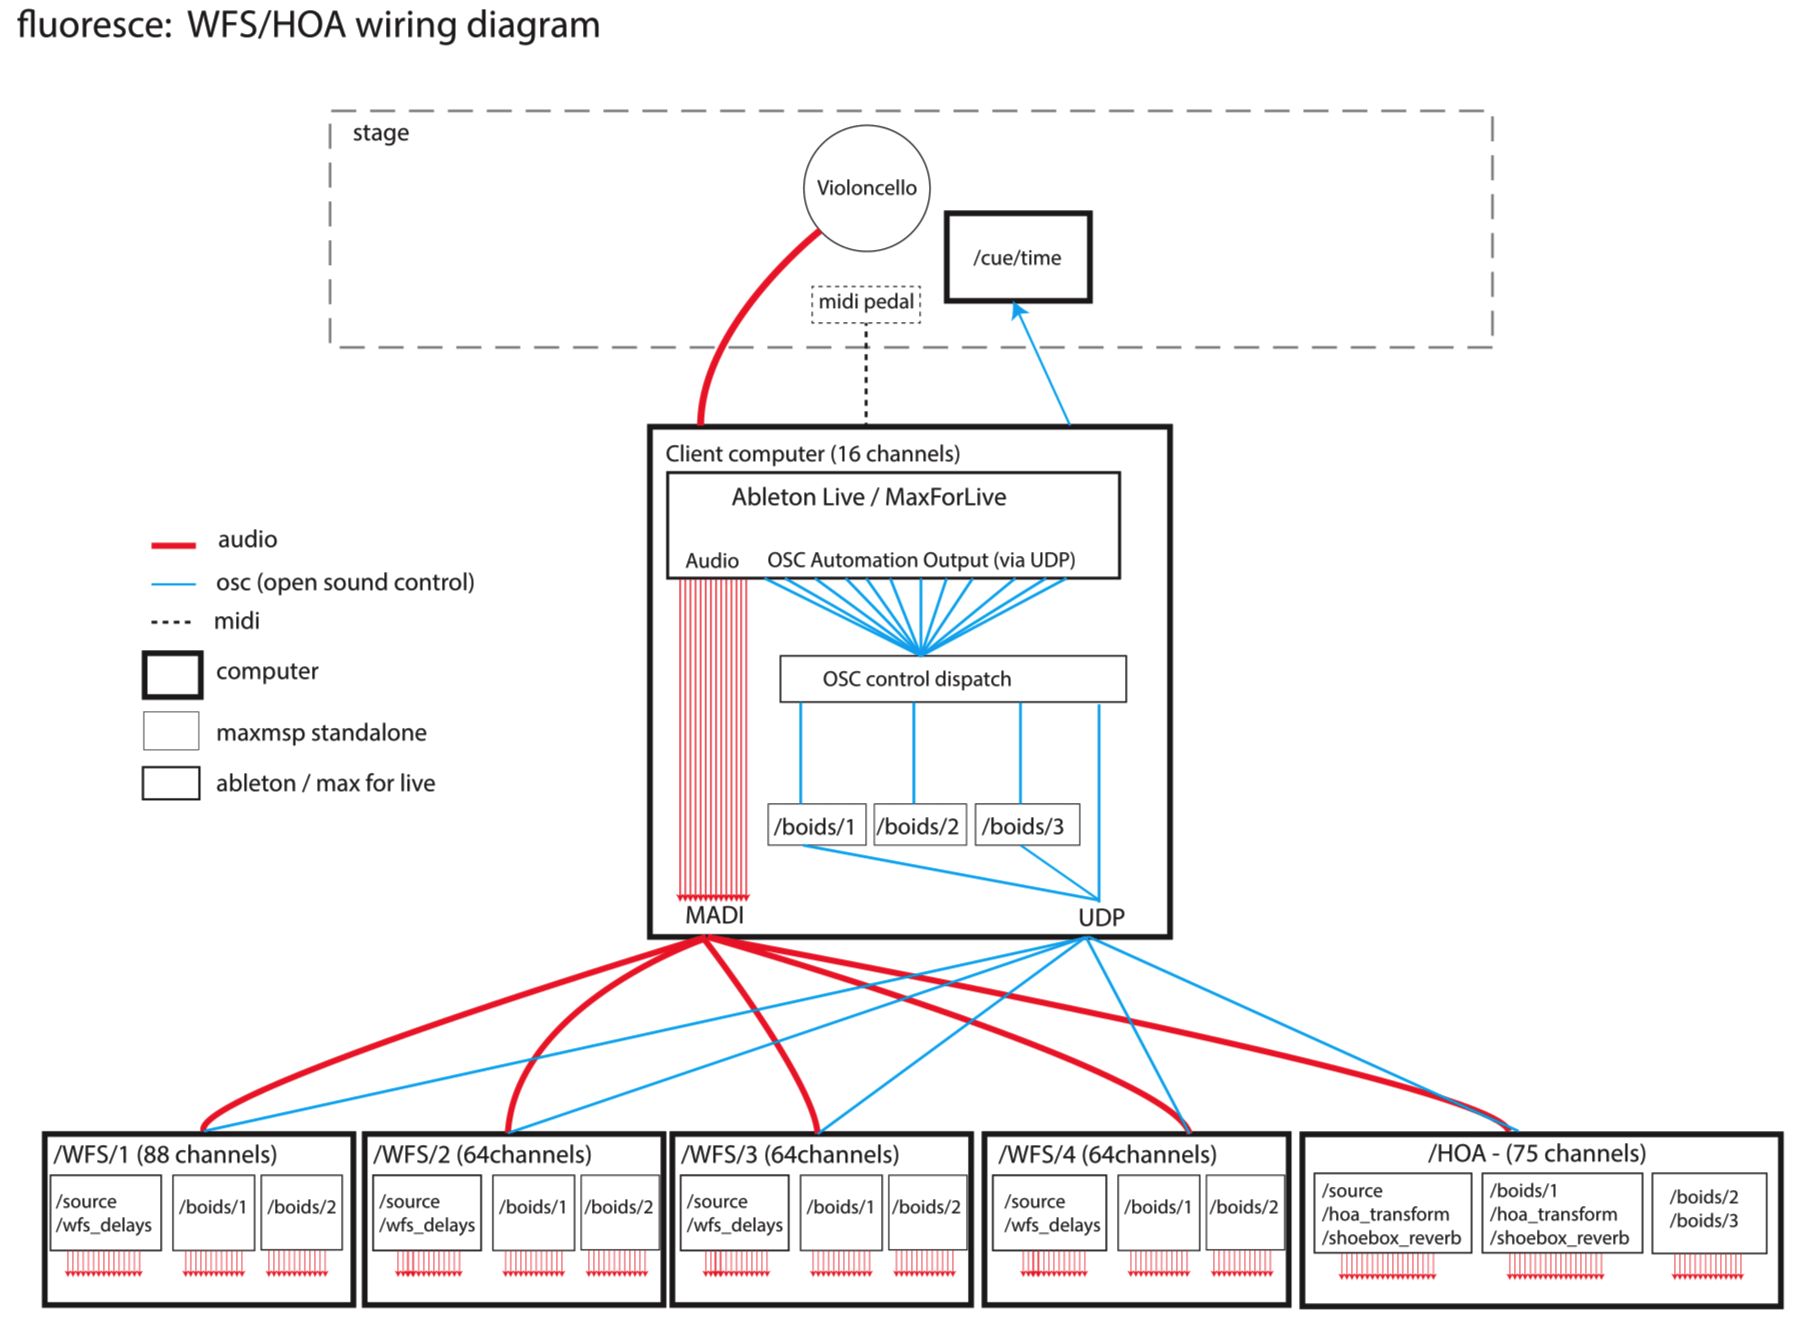
\includegraphics[keepaspectratio=true, width=\textwidth]{Annexes/i/schemaInstallationFluoresceComplet.png}
	\caption{Schéma complet de branchement pour la pièce \textit{Fluoresce}, Rama Gottfried, 2012}
	\label{fig:schemaInstallationFluoresceComplet}
\end{figure}
\begin{center}
\small
\it
La performance fait intervenir un joueur de violoncelle (Violoncello); le son produit par le violoncelle est capté et envoyé à un ordinateur (Client computer) sur lequel est lancé la station audionumérique (voir section \ref{subsec:stationAudionum}) Ableton Live associé au plugin MaxForLive\footnote{MaxForLive est un plugin permettant l'intégration de Max/MSP (voir section \ref{subsec:programmationVisuelle})} à la station audionumérique Ableton Live. Ableton Live va répartir le signal audio sur les systèmes WFS et HOA (Wave Field Synthesis et High Order Ambisonics\footnote{\textit{Wave Field Synthesis} et \textit{High Order Ambisonics} sont deux systèmes de diffusion de sons spatialisés basés sur l'utilisation d'un grand nombre d'enceintes.}) via la liaison MADI\footnote{MADI (Multichannel Audio Digital Interface) est une liaison audionumérique définissant un protocole capable d'embarquer 64 canaux audio simultanément}. Le plugin MaxForLive va s'occuper d'envoyer des messages OSC (voir section \ref{subsec:interoperabilite}) \texttt{/boids/1}, \texttt{/boids/2} et \texttt{/boids/3} (directives de déclenchement d'effets sonores), via UDP, aux systèmes WFS et HOA.
\end{center}

\section{Notation de la musique dans Max avec les libraires bach et dada}
\label{sec:exempleBachDada}
\begin{figure}[H]
	\centering
	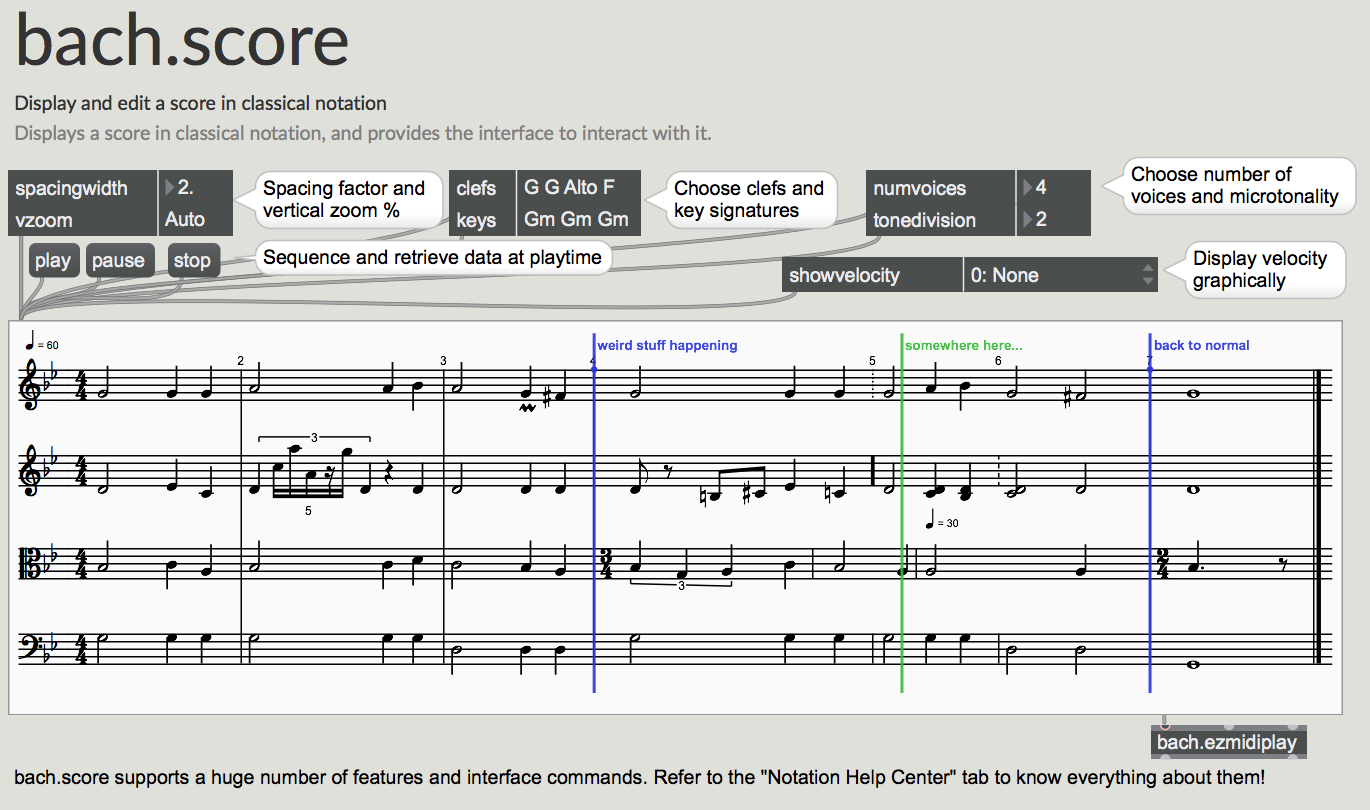
\includegraphics[keepaspectratio=true, height=0.45\textheight, width=\textwidth]{Annexes/i/exempleBachScore.png}
	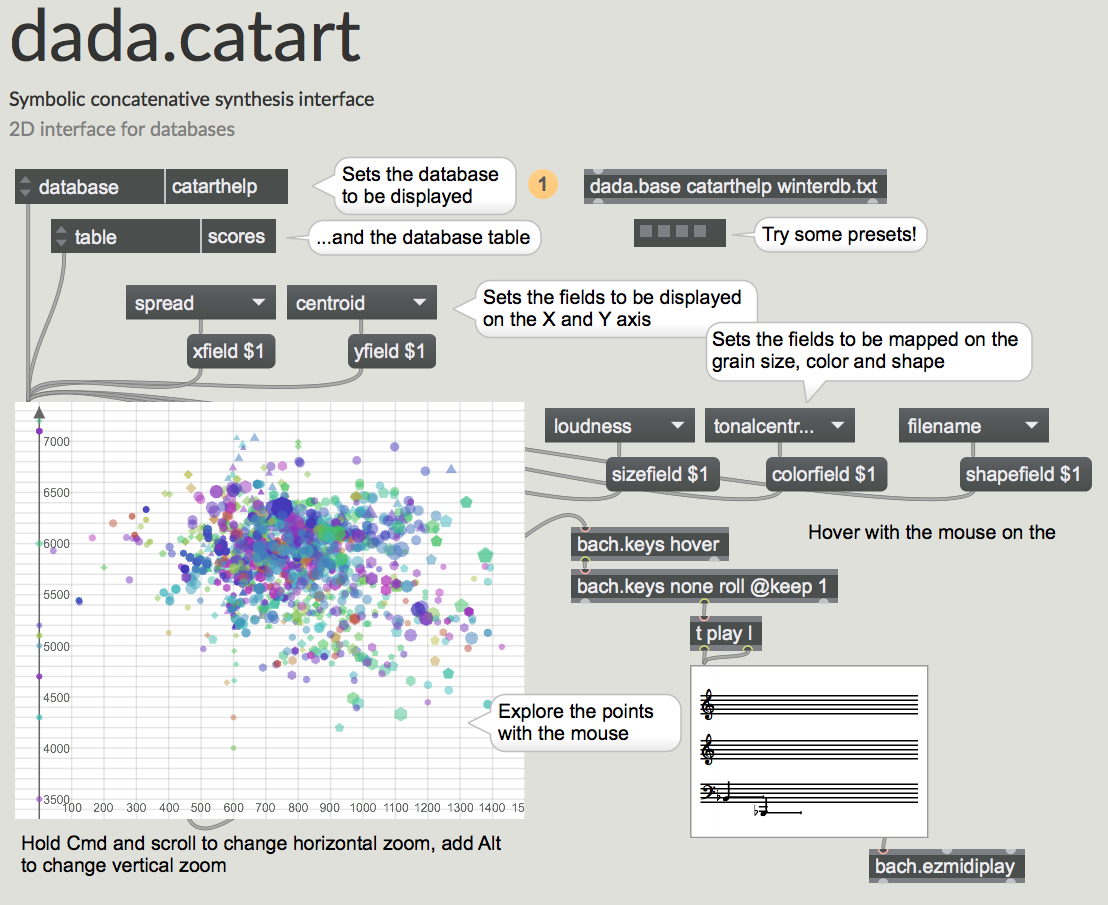
\includegraphics[keepaspectratio=true, height=0.45\textheight]{Annexes/i/exempleDadaCatart.png}
	\caption{Deux objets pour la notation de la musique dans Max : bach.score et dada.catart}
	\label{fig:exempleBachDada}
	\medskip
	\small
	\it 	
	Dans la figure du haut, la page de présentation de l'objet \textbf{bach.score} qui est un éditeur de notation traditionnelle, apportant une dimension de composition assistée par ordinateur au langage Max. Dans la figure du bas, la page de présentation de l'objet \textbf{dada.catart} qui permet de représenter la musique sous forme de nuages de points. L'exploration du nuage de points avec la souris fait apparaître la transcription en notation traditionnelle sur la portée en bas à droite.
\end{figure}

\section{Fragment de la pièce \textit{Lucky Wok}, Mike Solomon}
\label{sec:luckyWokSolomon}
\begin{figure}[H]
	\centering
	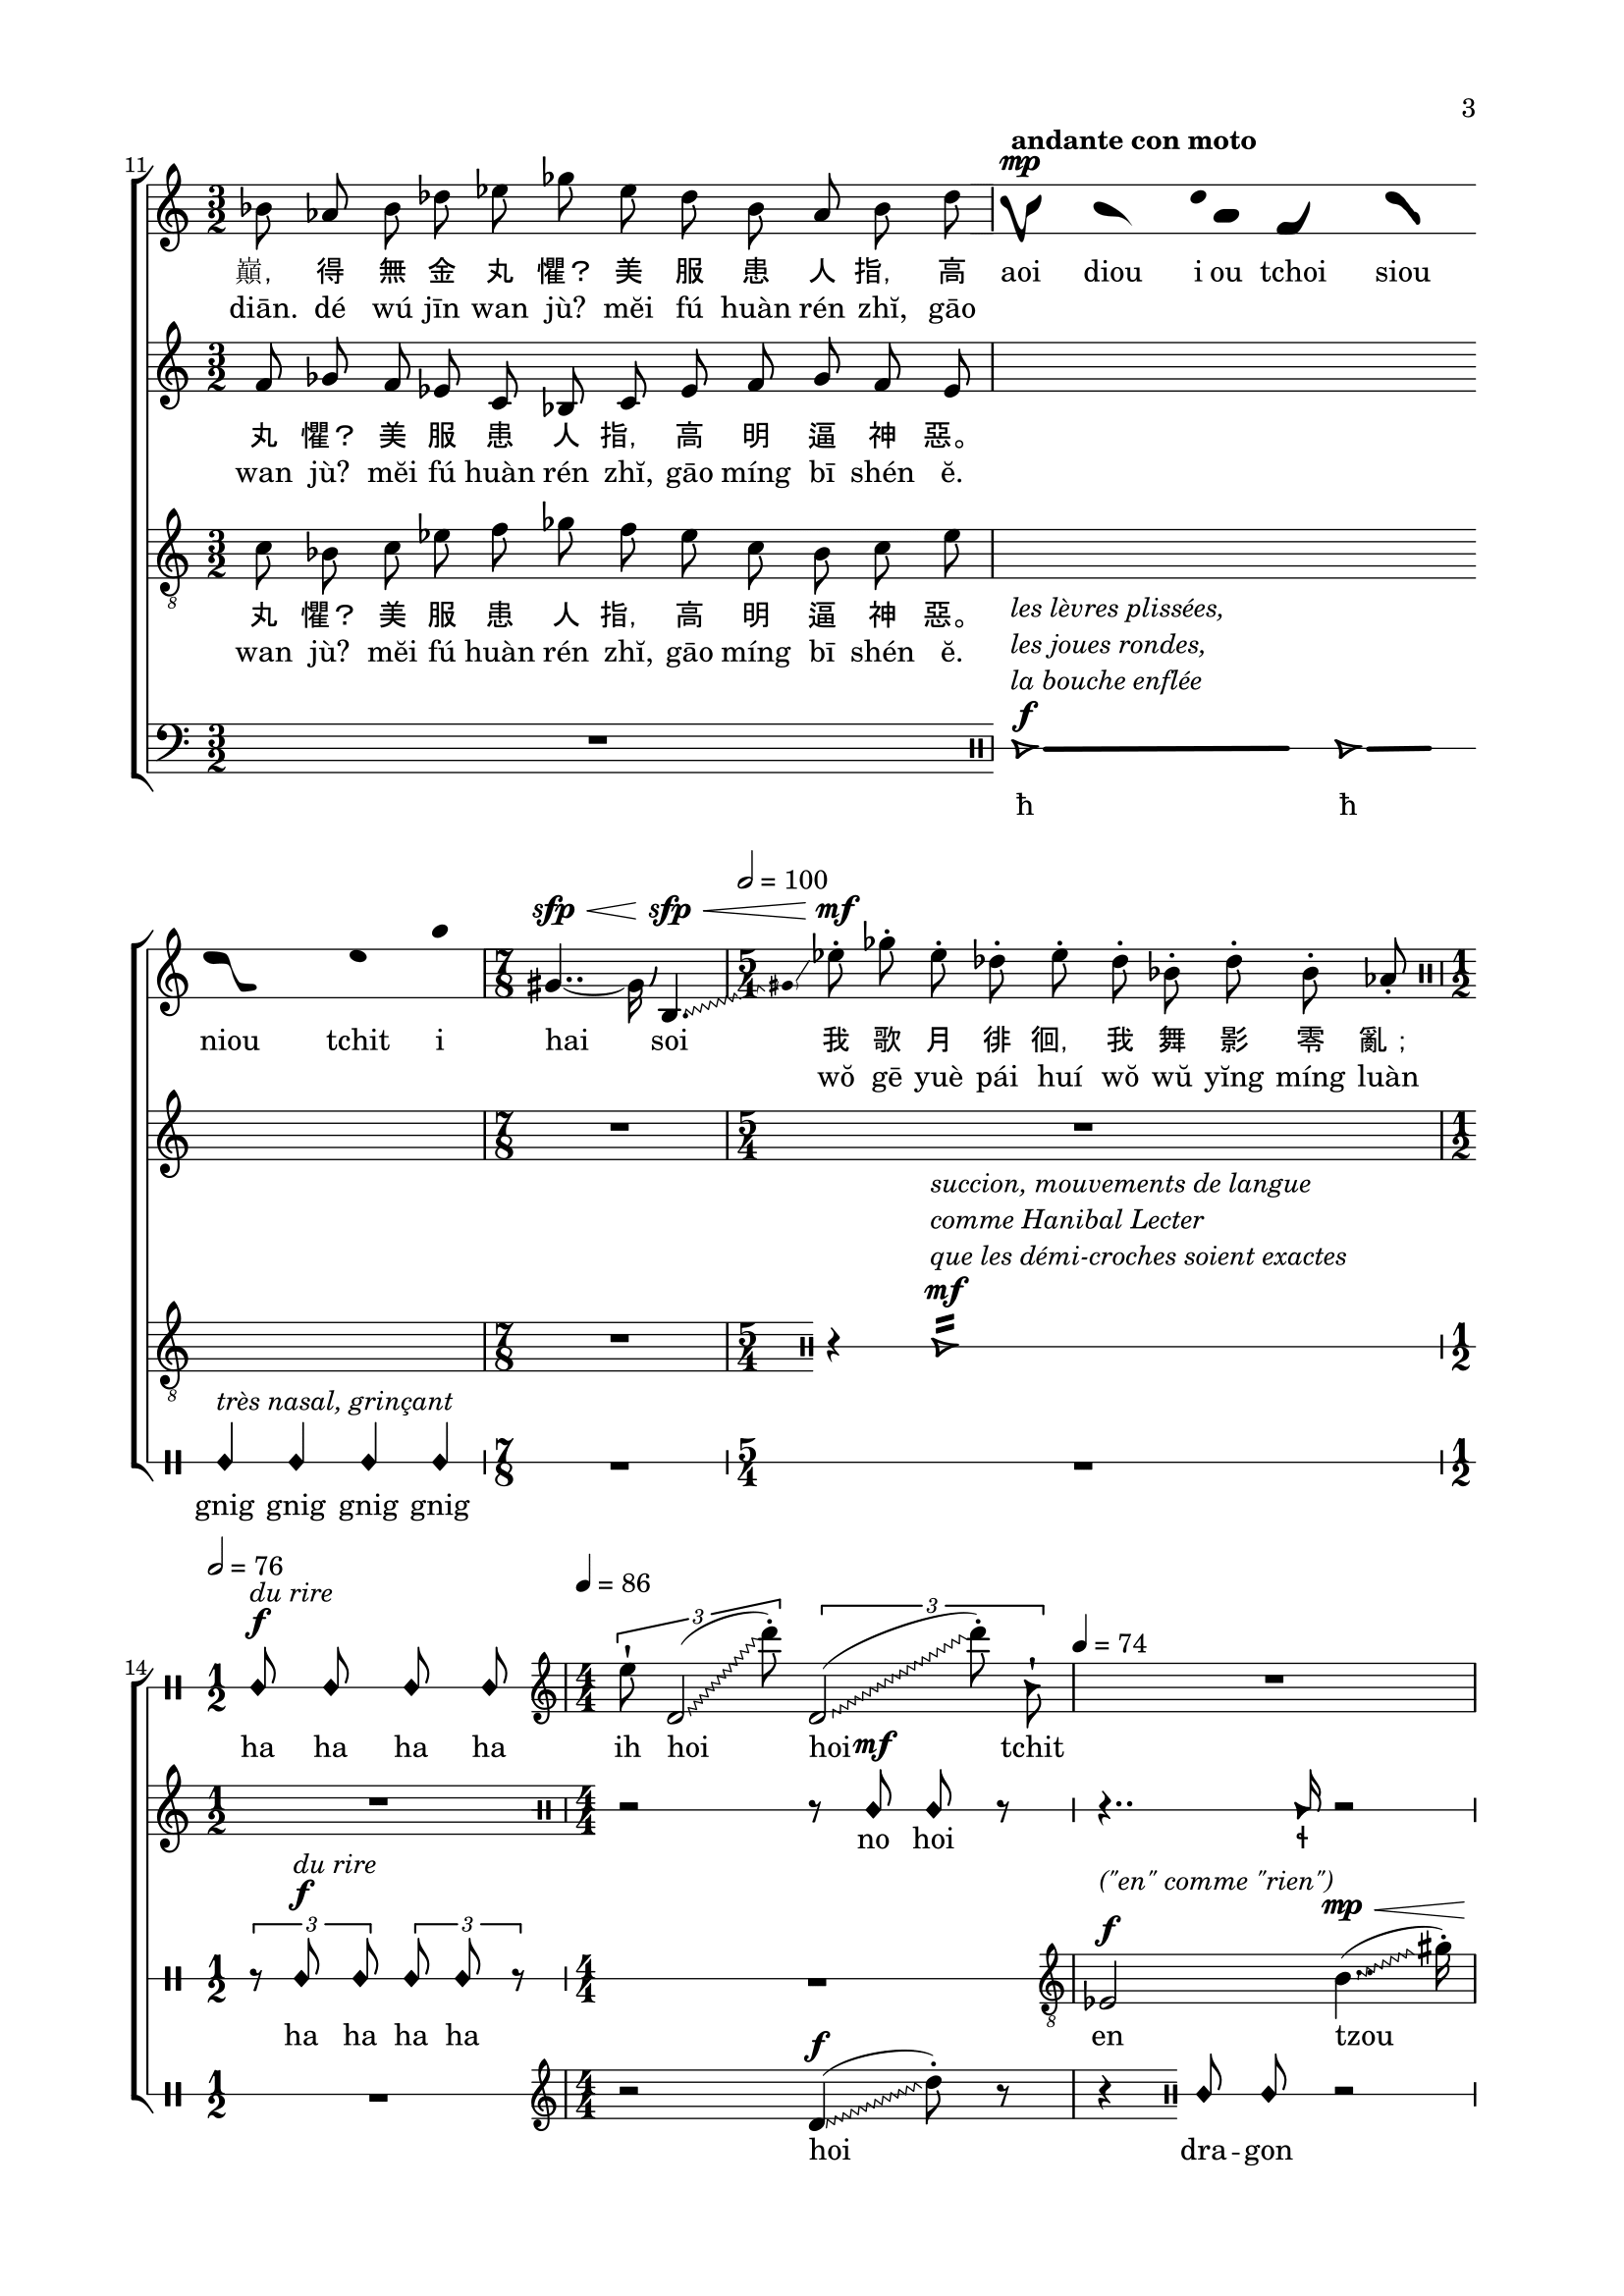
\includegraphics[keepaspectratio=true, width=0.92\textwidth]{Annexes/i/lucky.png}
	\caption{Fragment de la pièce \textit{Lucky Wok}, Mike Solomon}
	\medskip
	\small
	\it
	L'ensemble des symboles et effets de la partition sont produits avec Lilypond. 	
	\label{fig:luckyWokSolomon}
\end{figure}

\section{Exemple de partition créée avec IanniX}
\label{sec:exemplePartitionIannix}
\begin{figure}[H]
	\centering
	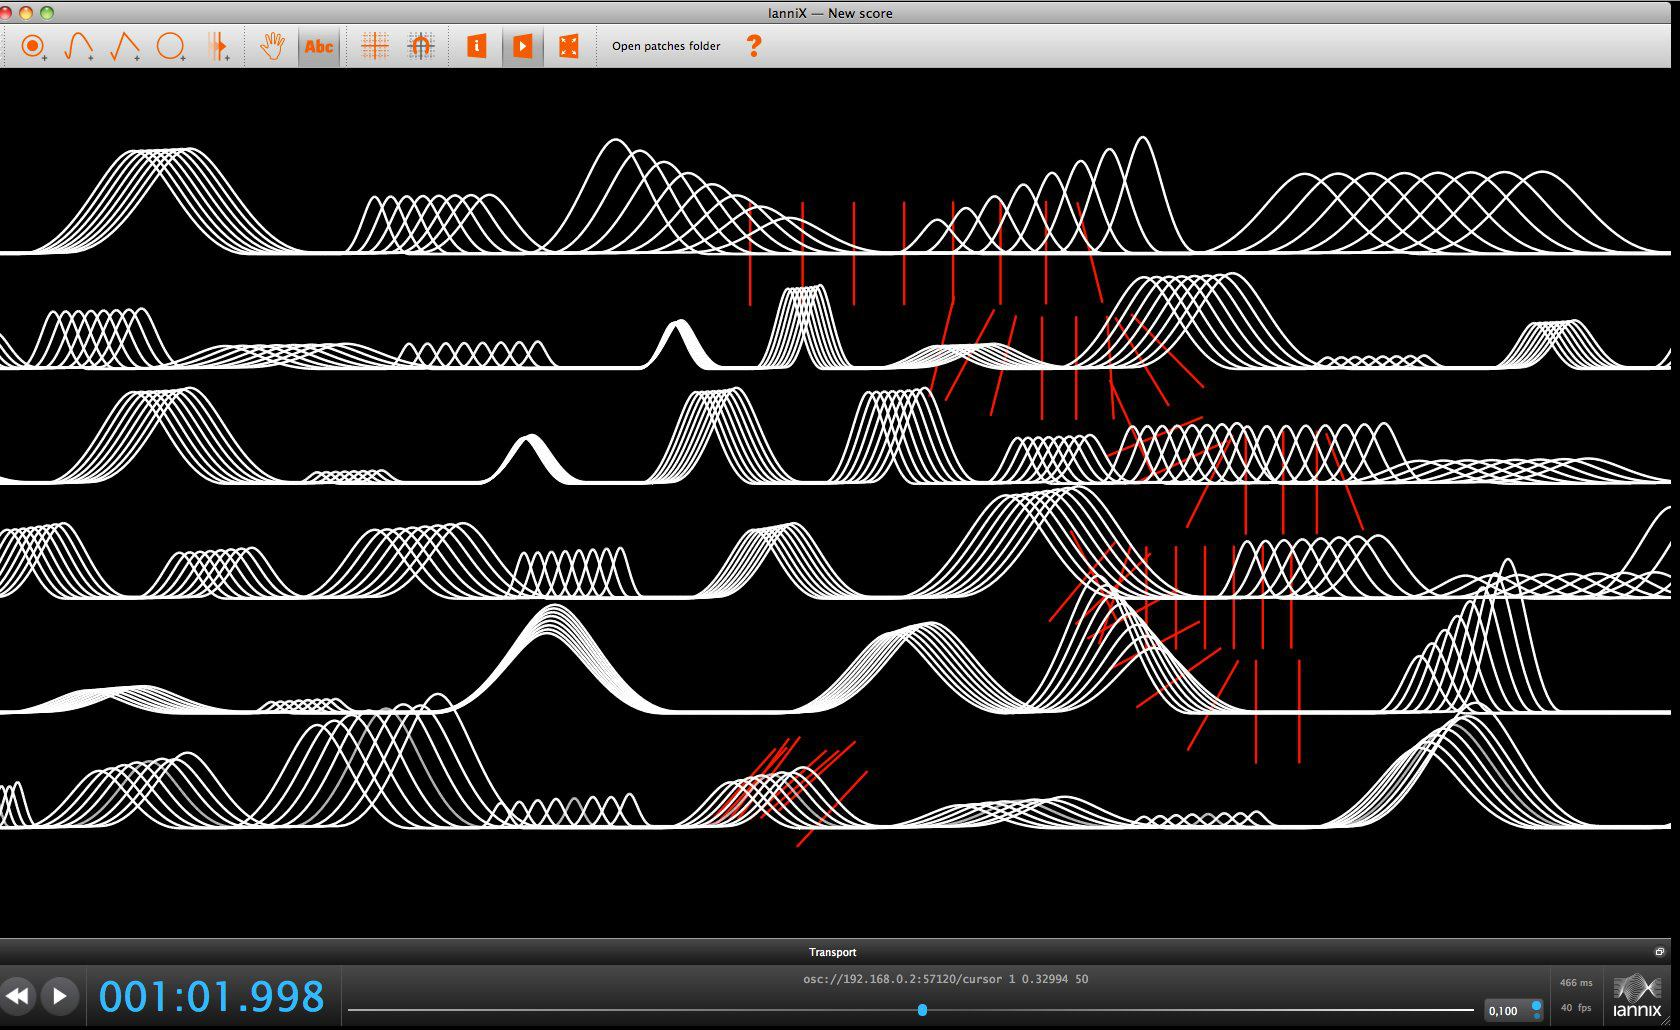
\includegraphics[keepaspectratio=true, width=0.92\textwidth]{Annexes/i/exemplePartitionIannix.jpg}
	\caption{Exemple de partition créée avec IanniX}
	\medskip
	\small
	\it
	Les barres rouges représentent les curseurs avançant le long des courbes blanches.
	Le caractère continue des courbes et leur superposition fait penser à une description morphologique de l'onde sonore. -- Source : Blog de Nicolas Boillot, \url{https://www.fluate.net/code/tools/} 	
	\label{fig:exemplePartitionIannix}
\end{figure}

\section{Exemple de partition interactive avec i-score}
\label{sec:exempleIScore}
\begin{figure}[H]
	\centering
	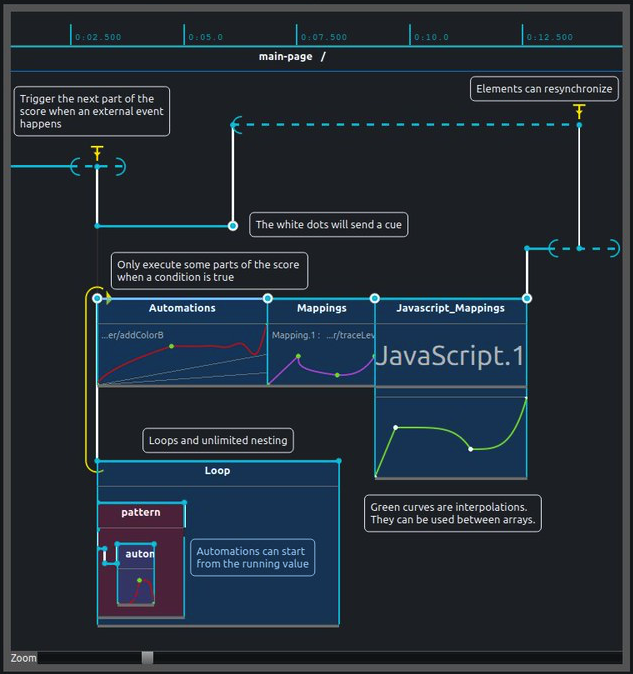
\includegraphics[keepaspectratio=true, width=\textwidth]{Annexes/i/exempleIScore.jpg}
	\caption{Exemple de partition interactive avec i-score}
	\medskip
	\small
	\it  	
	\label{fig:exempleIScore}
\end{figure}

\section{Vue d'une partition \textsc{INScore} et du script associé}
\label{sec:exempleINScore}
\begin{figure}[H]
	\centering
	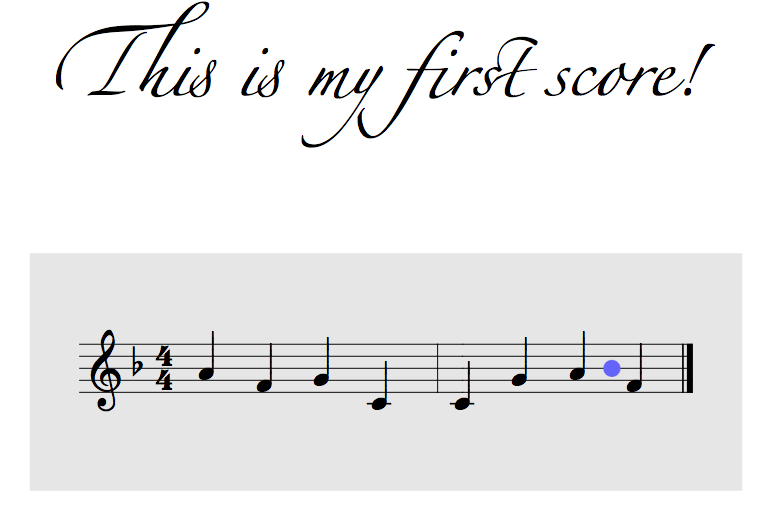
\includegraphics[keepaspectratio=true, width=\textwidth]{Annexes/i/exempleINScore.png}
	\begin{lstlisting}[language = python, linewidth = \textwidth]
# Suppression des précédents éléments de la scene
/ITL/scene/* del;

# Définition du titre de la scene
/ITL/scene/title set txt "This is my first score!";
/ITL/scene/title scale 3;
/ITL/scene/title y -0.6;
/ITL/scene/title fontFamily Zapfino;

# Mise en forme du cadre 
/ITL/scene/frame set rect 1.5 0.5;
/ITL/scene/frame color 230 230 230;

# Définition des notes de la portée
/ITL/scene/score set gmn '[ \meter<"4/4"> \key<-1> a f g c c g a f ]';
/ITL/scene/score scale 0.6;

# Création du curseur
/ITL/scene/cursor set ellipse 0.06 0.06;
/ITL/scene/cursor color 100 100 250;

# Synchronisation de l'objet score et cursor via l'objet sync
/ITL/scene/sync cursor score;

# Mise en mouvement du cursor le long de l'objet score
# via assignation d'une valeur de tempo
/ITL/scene/cursor tempo 60; 
	\end{lstlisting}
	\caption{Exemple de partition et de script \textsc{INScore}}
	\medskip
	\small
	\it
	La méthode \textbf{set gmn} (l.15) appelé sur l'objet \textbf{score} définit le contenu de la portée au format GUIDO. L'appel à l'objet \textbf{sync} (l.23) lie l'objet \textbf{cursor} et l'objet \textbf{score}. Ici, l'objet \textbf{cursor} devient esclave de l'objet \textbf{score}.  	
	\label{fig:exempleINScore}
\end{figure}

%\section{Vue de l'interface graphique de EAnalysis}
%\label{sec:exempleVueEAnalysis}
%\begin{figure}[H]
%	\centering
%	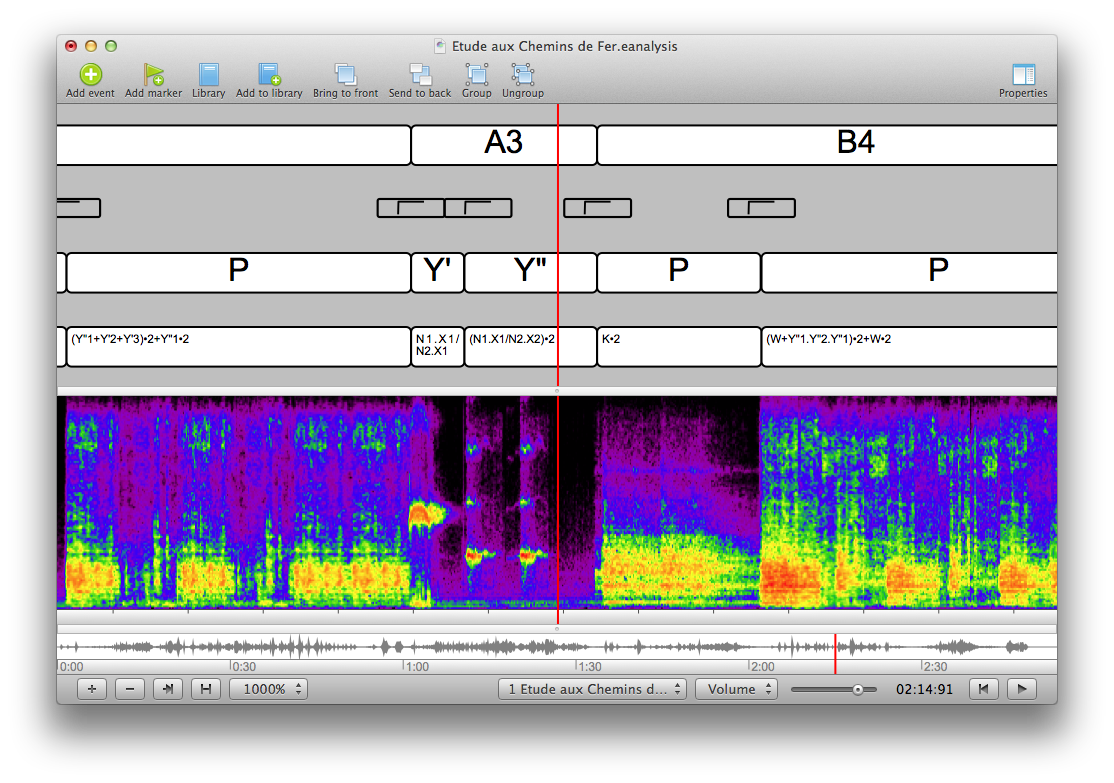
\includegraphics[keepaspectratio=true, width=0.92\textwidth]{Annexes/i/exempleVueEAnalysis.png}
%	\caption{Vue de l'interface graphique de EAnalysis}
%	\medskip
%	\small
%	\it
%	Plusieurs vues de la pièce \textit{Étude aux Chemins de Fer} dans l'environnement \textit{EAnalysis}.
%	De bas en haut : au premier niveau, la vue sous forme d'ondes; au deuxième niveau, le spectrogramme; au troisième niveau, la présentation des graphic et analytic events sur une ligne de temps parallèle.  	
%	\label{fig:exempleVueEAnalysis}
%\end{figure}